\documentclass[10pt]{beamer}

%Package
\usepackage[utf8]{inputenc}
\usepackage[absolute,overlay]{textpos}
% \usepackage[margin=1in]{geometry}
% \usepackage{amsmath}
% \usepackage{fancyhdr}
% \usepackage{graphicx}
% \usepackage{placeins}
% \usepackage{listings}
% \usepackage{color}
% \usepackage[table,xcdraw]{xcolor}
% \usepackage{ulem} %barrer du texte
% \usepackage{cancel}% barrer dans une expression math (\cancel{})
% \usepackage{pgf,tikz}
% \usepackage{mathrsfs}
% \usepackage{multirow}
%\usepackage{gensymb}
% \usepackage{caption}
% \usepackage{eurosym}% pour le symbole €


\usetheme{metropolis}           % Use metropolis theme
\title{Projet IF23 - GPS}

\date{17 Juin 2016}
\author{Thomas Jeantet - Geoffrey Gaillard}
\institute{Université de Technologie de Troyes}

\begin{document}

	\maketitle
	\section{Fonctionalité du GPS}
	\begin{frame}{Le boitier}

		\begin{textblock*}{80mm}(2.5mm,10mm)
			\begin{block}{LCD}
			Donnée disponible sur le LCD :
			\begin{itemize}
				\item Latitude
				\item Longitude
				\item Nombre de satellites visibles
				\item HDOP
				\item Altitude
				\item Vitesse
				\item Date
				\item Heure GPS
				\item Tension de la batterie
				\item Autonomie en heures
				\item Pourcentage de charge de la batterie
			\end{itemize}
			\end{block}
		\end{textblock*}
		
		\begin{textblock*}{60mm}(67.5mm,10mm)
			\begin{block}{Fonctionalité}
			\begin{itemize}
				\item Prise de points
				\item Prise d'itinéraire
			\end{itemize}
			Minimisation des fonctionalités au sien du boitier pour une cause :
			\begin{itemize}
				\item Limitation RAM
				\item Limitation Mémoire
			\end{itemize}
			\end{block}
		\end{textblock*}
	\end{frame}

	\begin{frame}{Elementaire GPS}
		\begin{textblock*}{80mm}(2.5mm,60mm)
			\begin{itemize}
				\item Permet le transfert du boitier à l'ordinateur 
				\item La gestion des fichiers sur le boitier 
				\item Le traitment des données recoltées et transfert depuis le boitier
				\item Conversion des données en format GPX
			\end{itemize}
		\end{textblock*}

		\begin{textblock*}{80mm}(20mm,12.5mm)
				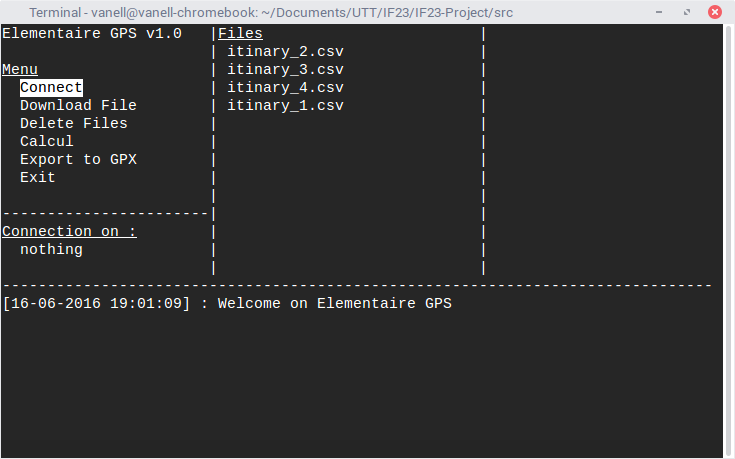
\includegraphics[width=225px]{elementaire_gps.png}
		\end{textblock*}
		
	\end{frame}

	\section{Les Mesures}

  \begin{frame}{Lieux des mesures}
  		\begin{textblock*}{60mm}(2.5mm,15mm)
	  		\begin{block}{Appartement}
				Appartement au 1er etage d’un immeuble : Batiments en béton autour, prise de points à la fenêtre.\\ Mesure de nuit.
			\end{block}
  		\end{textblock*}

  		 \begin{textblock*}{61mm}(67.5mm,15mm)
  		 	\begin{block}{Terrasse}
				Terrasse de la salle associative de l’UTT\\ Dans un recoin, entre deux murs métalliques de l’UTT.\\ Météo ensoleillée.
			\end{block}
  		\end{textblock*}

  		\begin{textblock*}{60mm}(2.5mm,50mm)
  		 	\begin{block}{Voiture}
				Voiture a l’arrêt dans le parking de l’UTT : environnement métallique moins important que la terrasse. Météo ensoleillée.
			\end{block}
  		\end{textblock*}


		\begin{textblock*}{60mm}(67.5mm,50mm)
			\begin{block}{Colline}
				Colline dégagée. Météo ensoleillée puis orageuse.
			\end{block}
		\end{textblock*}
  \end{frame}
  
  \begin{frame}{Compartif globale des données}

    		\begin{textblock*}{60mm}(2.5mm,12.5mm)
	  		\begin{block}{Appartement}
				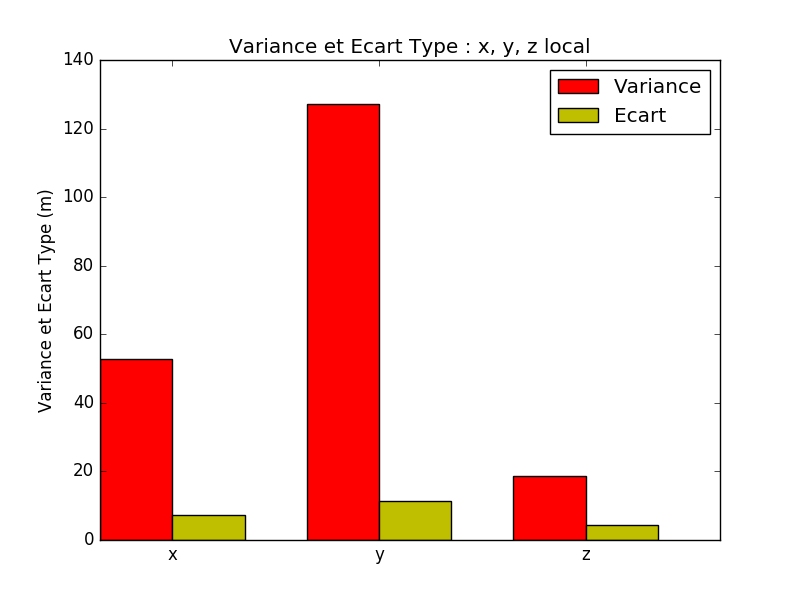
\includegraphics[width=125px]{../src/data/itinary_1/var_ecart1.png}
			\end{block}
  		\end{textblock*}

  		 \begin{textblock*}{60mm}(70mm,12.5mm)
  		 	\begin{block}{Terrasse}
				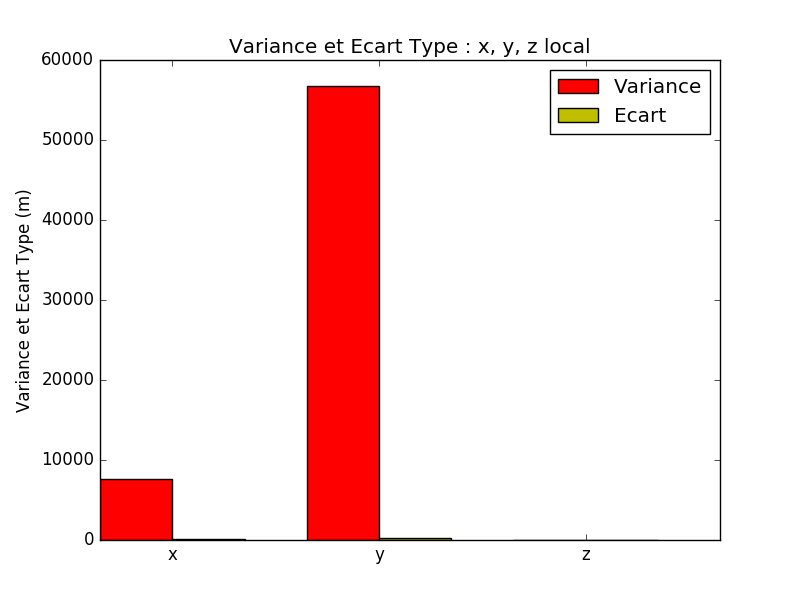
\includegraphics[width=125px]{../src/data/itinary_2/var_ecart2.png}
			\end{block}
  		\end{textblock*}

  		\begin{textblock*}{60mm}(2.5mm,52.5mm)
  		 	\begin{block}{Voiture}
				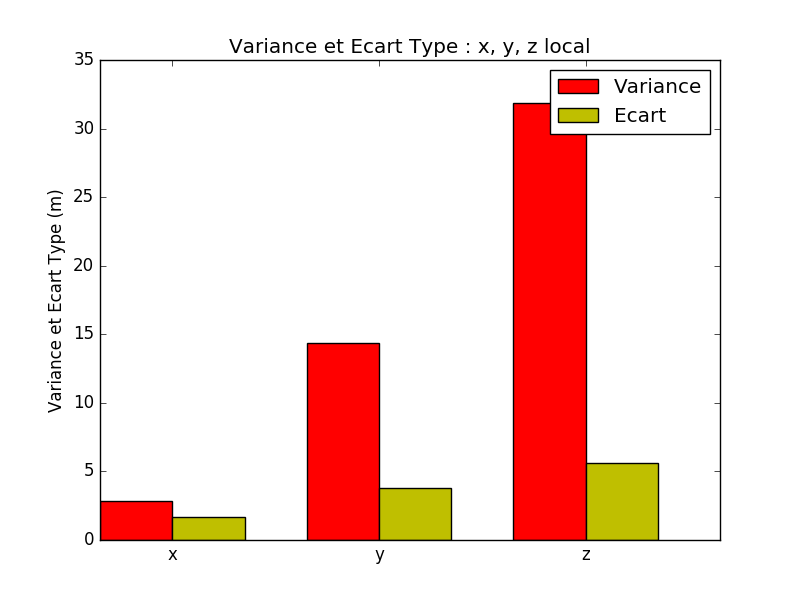
\includegraphics[width=125px]{../src/data/itinary_3/var_ecart3.png}
			\end{block}
  		\end{textblock*}


		\begin{textblock*}{60mm}(70mm,52.5mm)
			\begin{block}{Colline}
				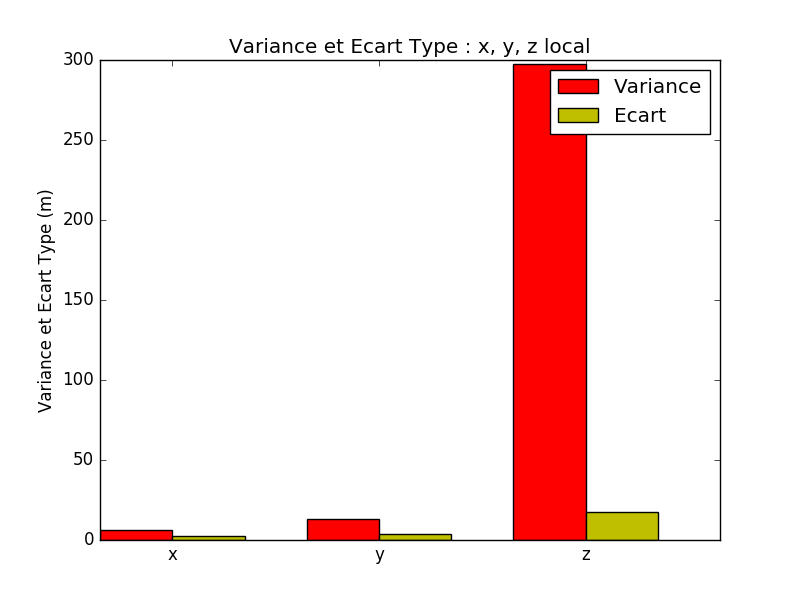
\includegraphics[width=125px]{../src/data/itinary_4/var_ecart4.png}
			\end{block}
		\end{textblock*}
  \end{frame}

	\begin{frame}{Appartement}

		\begin{textblock*}{60mm}(2.5mm,12.5mm)
			\begin{block}{$x$ local}
				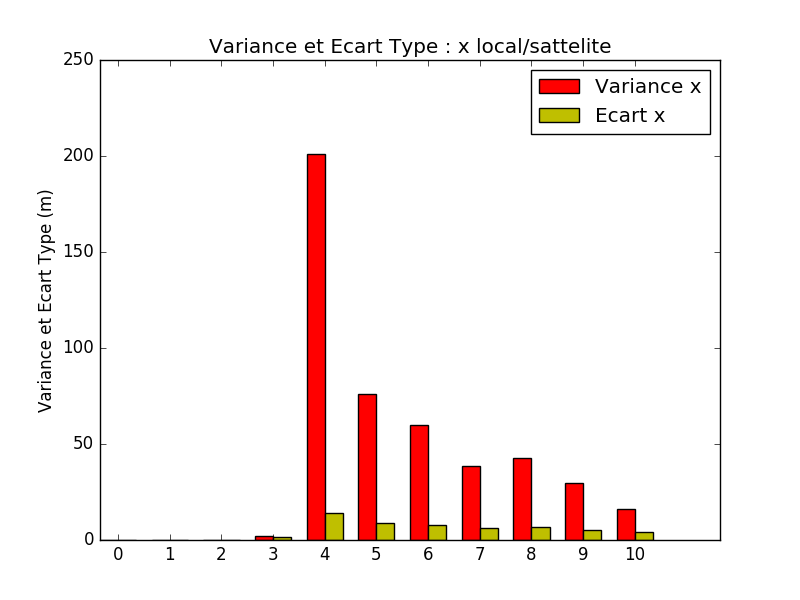
\includegraphics[width=125px]{../src/data/itinary_1/var_ecart_sat_x1.png}
			\end{block}
		\end{textblock*}

		\begin{textblock*}{60mm}(70mm,12.5mm)
			\begin{block}{$y$ local}
				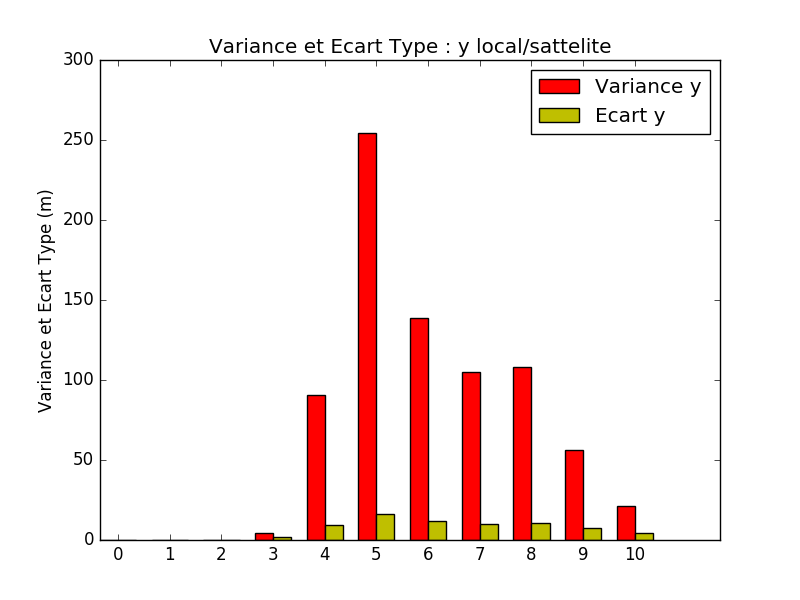
\includegraphics[width=125px]{../src/data/itinary_1/var_ecart_sat_y1.png}
			\end{block}
		\end{textblock*}

		\begin{textblock*}{60mm}(0.35\textwidth,52.5mm)
			\begin{block}{$z$ local}
				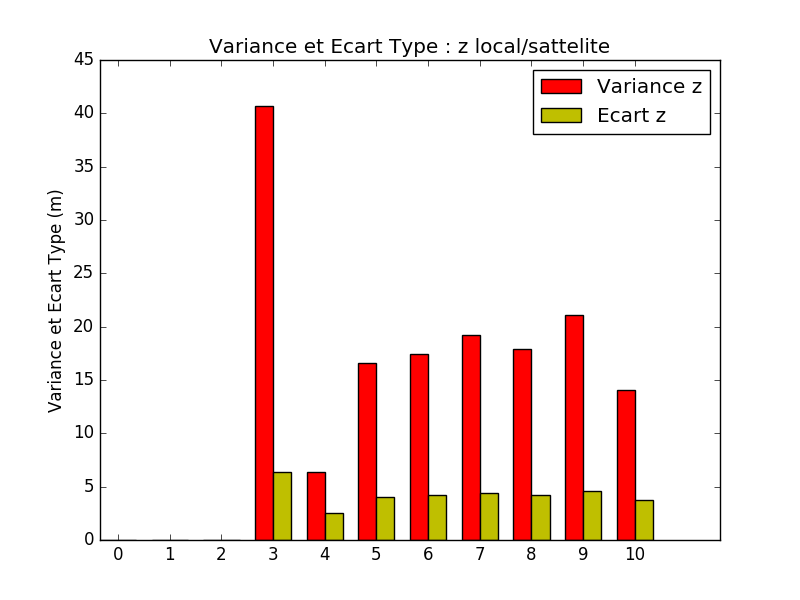
\includegraphics[width=125px]{../src/data/itinary_1/var_ecart_sat_z1.png}
			\end{block}
		\end{textblock*}
	\end{frame}

	\begin{frame}{Terrasse}
		\begin{textblock*}{60mm}(2.5mm,12.5mm)
			\begin{block}{$x$ local}
				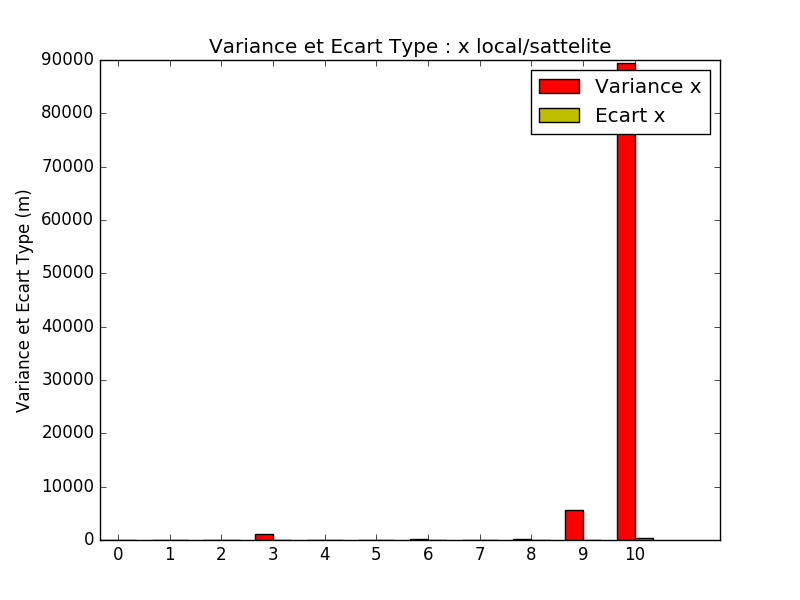
\includegraphics[width=125px]{../src/data/itinary_2/var_ecart_sat_x2.png}
			\end{block}
		\end{textblock*}

		\begin{textblock*}{60mm}(70mm,12.5mm)
			\begin{block}{$y$ local}
				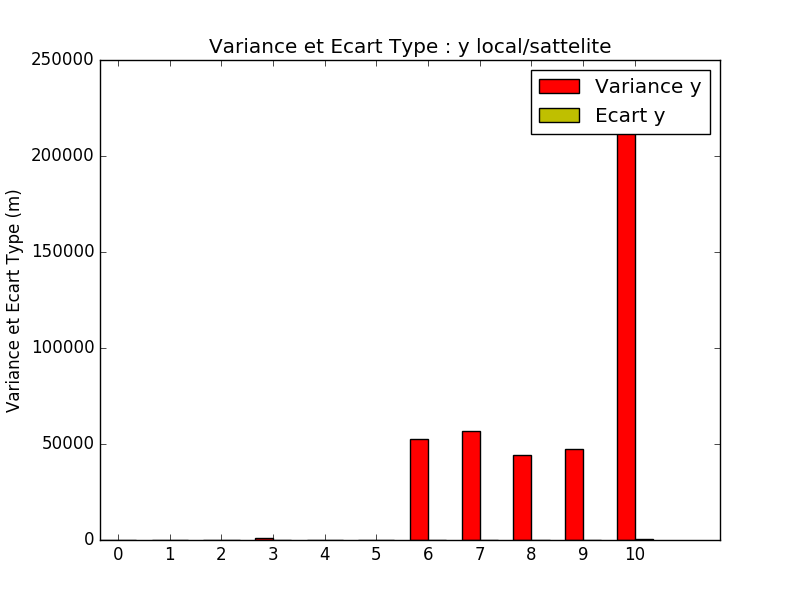
\includegraphics[width=125px]{../src/data/itinary_2/var_ecart_sat_y2.png}
			\end{block}
		\end{textblock*}

		\begin{textblock*}{60mm}(0.35\textwidth,52.5mm)
			\begin{block}{$z$ local}
				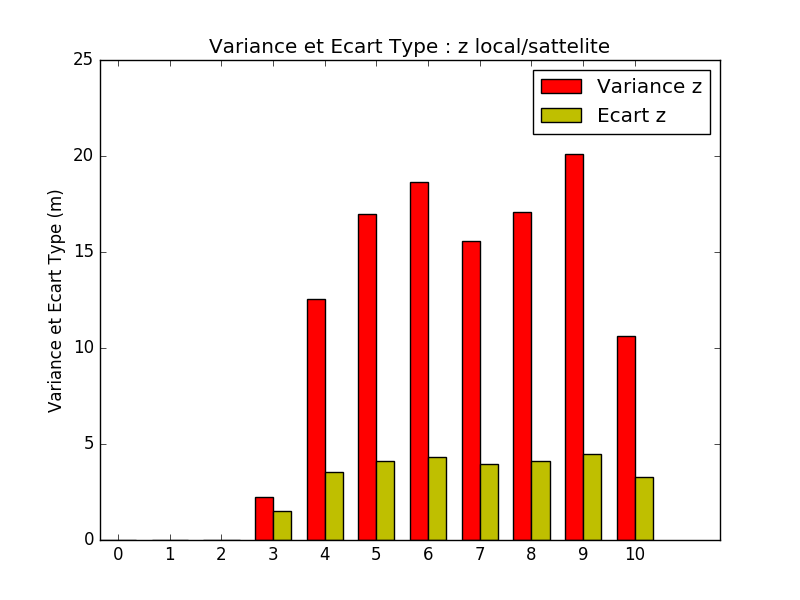
\includegraphics[width=125px]{../src/data/itinary_2/var_ecart_sat_z2.png}
			\end{block}
		\end{textblock*}
	\end{frame}

	\begin{frame}{Voiture}
		\begin{textblock*}{60mm}(2.5mm,12.5mm)
			\begin{block}{$x$ local}
				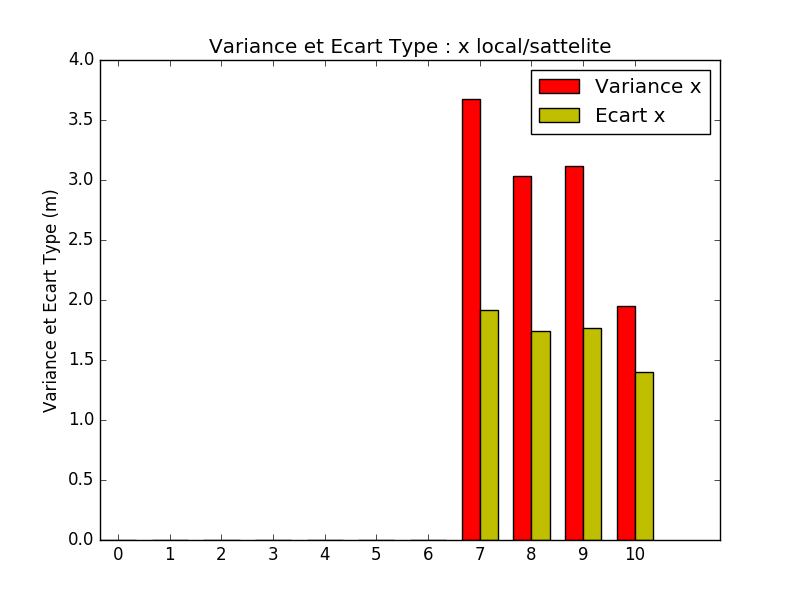
\includegraphics[width=125px]{../src/data/itinary_3/var_ecart_sat_x3.png}
			\end{block}
		\end{textblock*}

		\begin{textblock*}{60mm}(70mm,12.5mm)
			\begin{block}{$y$ local}
				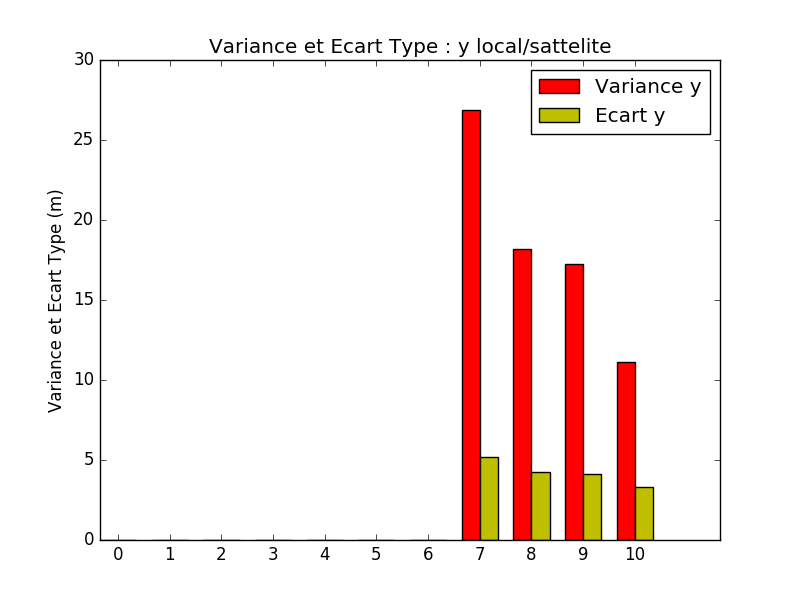
\includegraphics[width=125px]{../src/data/itinary_3/var_ecart_sat_y3.png}
			\end{block}
		\end{textblock*}

		\begin{textblock*}{60mm}(0.35\textwidth,52.5mm)
			\begin{block}{$z$ local}
				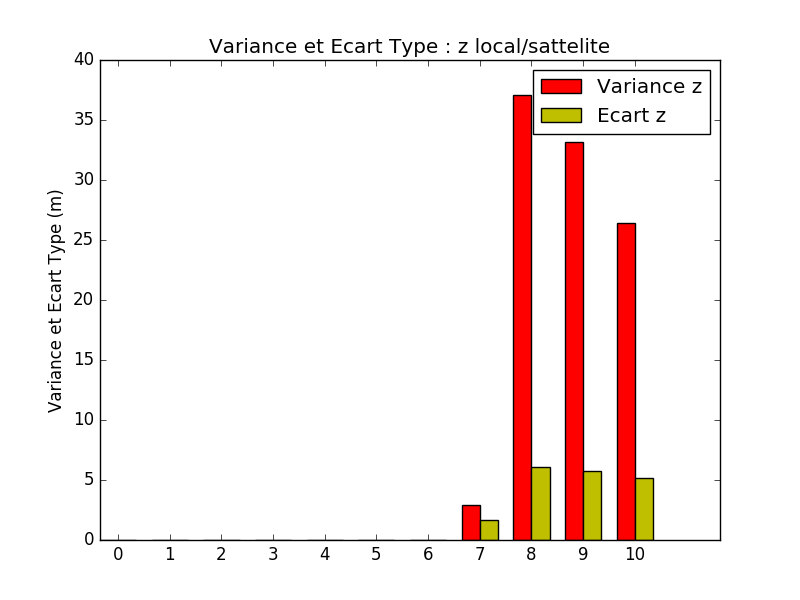
\includegraphics[width=125px]{../src/data/itinary_3/var_ecart_sat_z3.png}
			\end{block}
		\end{textblock*}
	\end{frame}

	\begin{frame}{Colline}
		\begin{textblock*}{60mm}(2.5mm,12.5mm)
			\begin{block}{$x$ local}
				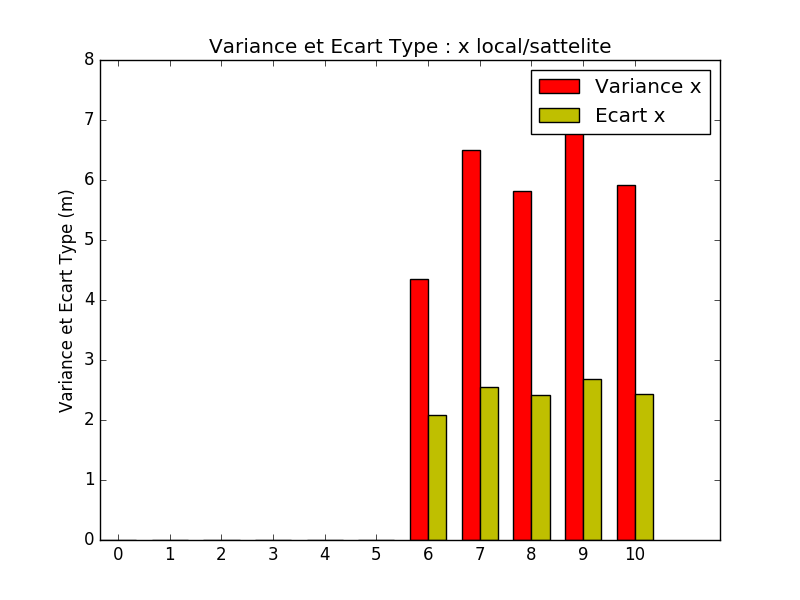
\includegraphics[width=125px]{../src/data/itinary_4/var_ecart_sat_x4.png}
			\end{block}
		\end{textblock*}

		\begin{textblock*}{60mm}(70mm,12.5mm)
			\begin{block}{$y$ local}
				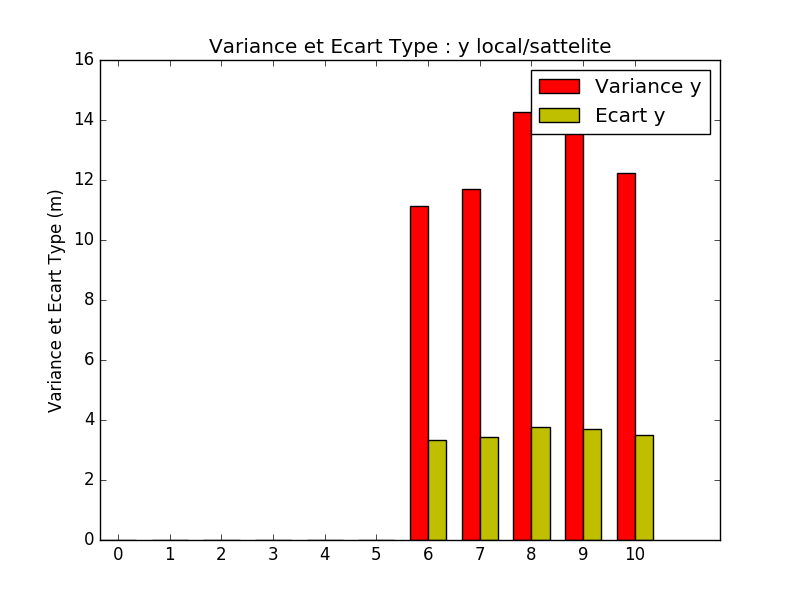
\includegraphics[width=125px]{../src/data/itinary_4/var_ecart_sat_y4.png}
			\end{block}
		\end{textblock*}

		\begin{textblock*}{60mm}(0.35\textwidth,52.5mm)
			\begin{block}{$z$ local}
				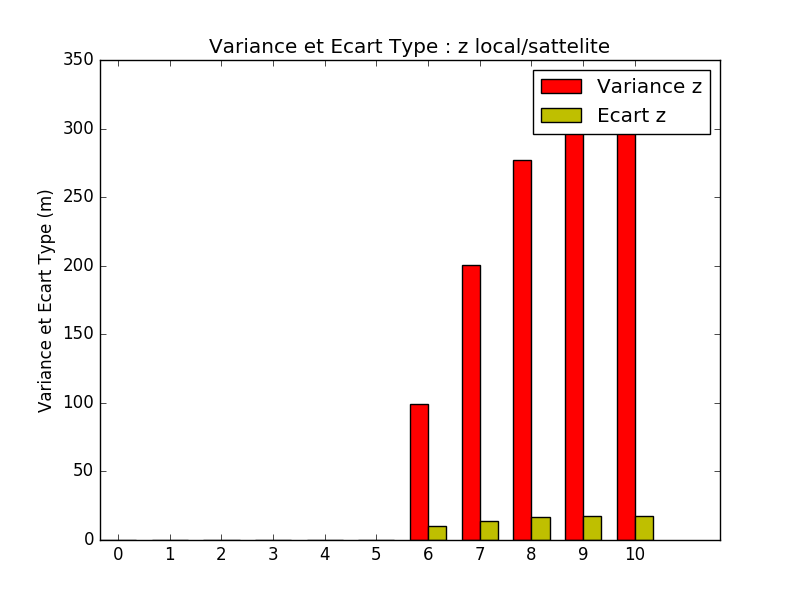
\includegraphics[width=125px]{../src/data/itinary_4/var_ecart_sat_z4.png}
			\end{block}
		\end{textblock*}
	\end{frame}

	\begin{frame}{Lambert 93}
	    \begin{textblock*}{60mm}(2.5mm,12.5mm)
	  		\begin{block}{Appartement}
				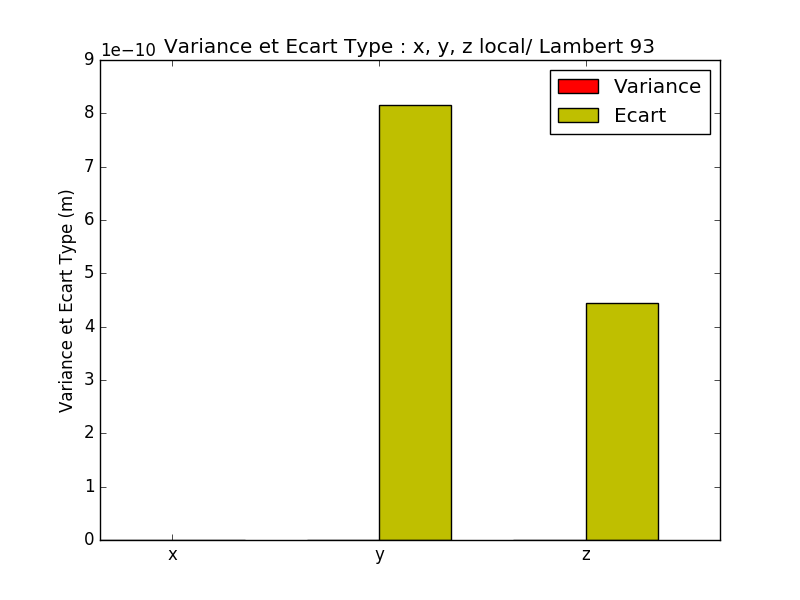
\includegraphics[width=125px]{../src/data/itinary_1/var_ecart_lambert1.png}
			\end{block}
  		\end{textblock*}

  		 \begin{textblock*}{60mm}(70mm,12.5mm)
  		 	\begin{block}{Terrasse}
				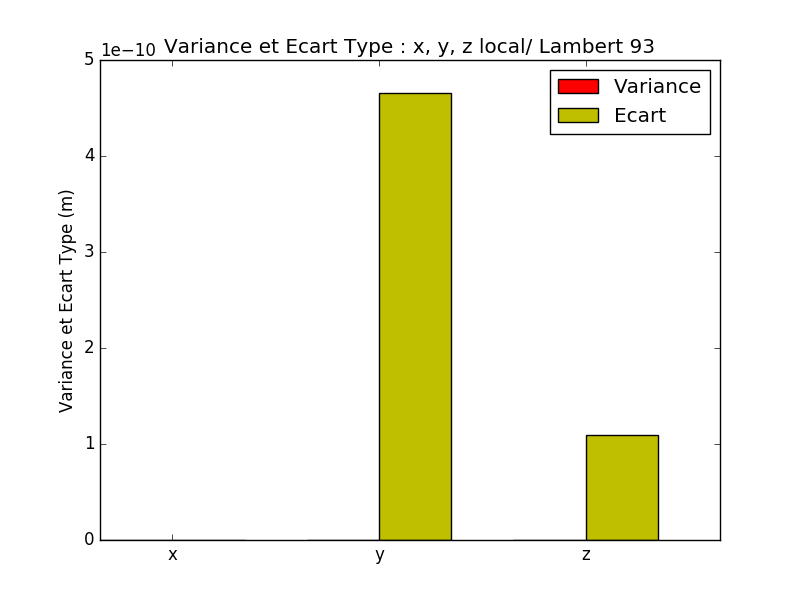
\includegraphics[width=125px]{../src/data/itinary_2/var_ecart_lambert2.png}
			\end{block}
  		\end{textblock*}

  		\begin{textblock*}{60mm}(2.5mm,52.5mm)
  		 	\begin{block}{Voiture}
				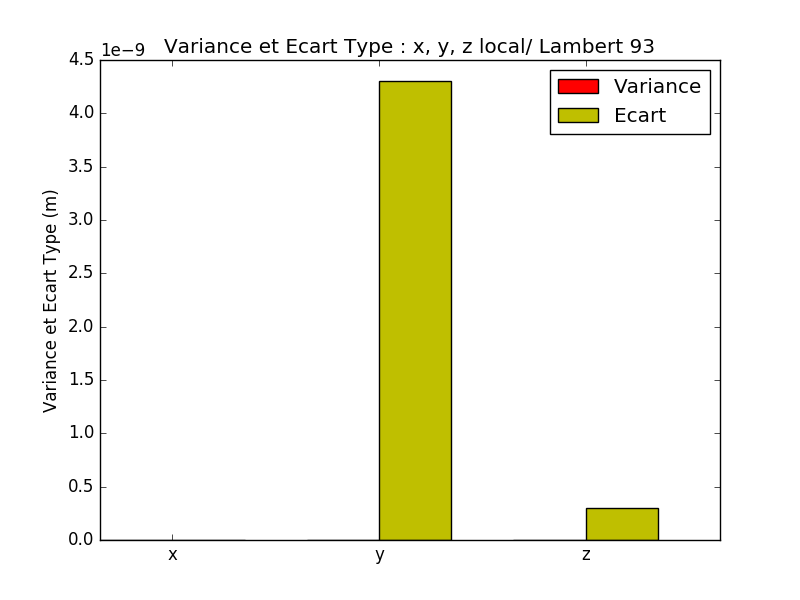
\includegraphics[width=125px]{../src/data/itinary_3/var_ecart_lambert3.png}
			\end{block}
  		\end{textblock*}


		\begin{textblock*}{60mm}(70mm,52.5mm)
			\begin{block}{Colline}
				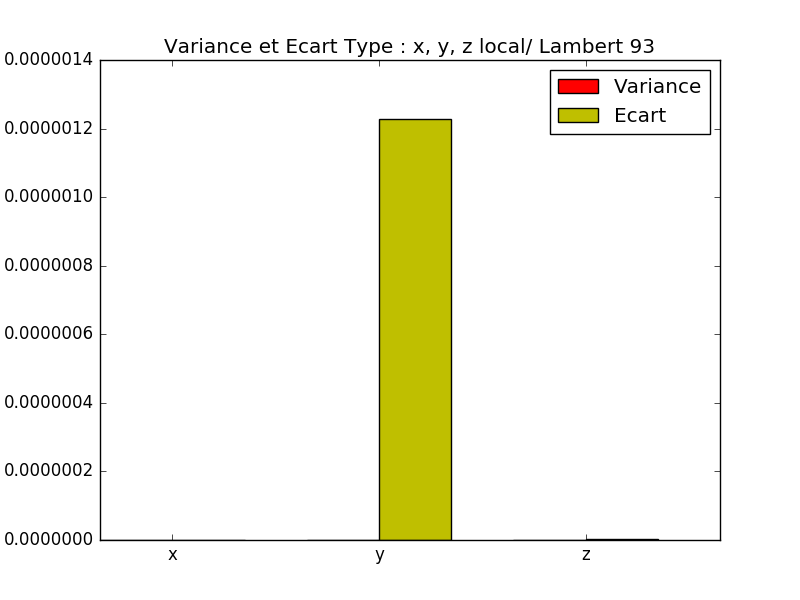
\includegraphics[width=125px]{../src/data/itinary_4/var_ecart_lambert4.png}
			\end{block}
		\end{textblock*}
	\end{frame}

	\section{Conclusion}
	\section{Question ?}
\end{document}